\chapter{Aspektorientierte Programmierung}
\label{chap:aop}

\section{Geschichte}
\label{sec:aop_geschichte}

Das Konzept der Aspektorientierten Programmierung wurde im Xerox PARC (Palo Alto Research Center Incorporated) entwickelt und gewann ab 1995 an Wichtigkeit. Wie bei allen neuen Spezifikationen war der Umfang und die Bestandteile der Aspektorientierten Programmierung zuerst nicht klar abgegrenzt. Gregor Kiczales und sein Team waren massgeblich an der Entwicklung von AOP beteiligt.\\
Nach Entwicklung des theoretischen Grundlage folgte im Jahre 1998 eine erste Version von AspectJ, eine Implementation von AOP in Java. Die Version 1.0 von AspectJ wurde jedoch erst im Jahre 2002 nach weiterer Forschung veröffentlicht.\cite{lopes:historyaop} \\
Die Aspektorientierte Programmierung wurde durch die Publikation von AspectJ bekannt und es wurden seither Erweiterungen für die meisten populären Programmiersprachen entwickelt. 

Die Entwicklung und der Betrieb von AspectJ wurde von XeroX Parc an Eclipse weitergereicht. Dort läuft AspectJ bis heute als Open-Source Projekt weiter. Mit der Version 1.8.7 wurde am 9. September 2015 die aktuellste Version veröffentlicht.

\section{Motivation}
\label{sec:aop_motivation}

Einer der Hauptgründe warum AOP entwickelt wurde ist die erweiterte Modularität die damit erreicht werden kann. Beim Design eines Systems werden in der Regel verschiedene Kategorien von Funktionalitäten aufgestellt und so die Software in verschiedene sogenannte Anliegen aufgeteilt. Dabei unterscheidet man zwischen den folgenden zwei Gruppen:

\begin{itemize}
	\item Kernanliegen (core concerns)\\
	Hierbei handelt sich um die Kernfunktionalität der Applikation, die sogenannte Business Logic. Diese Gruppe beinhaltet zum Beispiel den Datenbankzugriff, die Interagierung mit dem Benutzer etc.
	\item System Übergreifende Anliegen (cross-cutting concerns \\
	Andere Funktionalitäten wie das Logging, die Sicherheit, Concurrency sowie Transaktionen betreffen das gesamte System.
\end{itemize}

Diese Gruppen dienen als Grundlage zur Veranschaulichung, warum gerade bei der Modularisierung die OOP Schwachstellen aufweist.

\subsection{Objektoriente Programmierung}
\label{sec:aop_oop}

Mit der Objektorientierten Programmierung wurden viele Probleme und Unschönheiten von Prozeduralen Sprachen gelöst. Die OOP besitzt riesige Vorteile, welche die Softwareentwicklung vereinfachen. Einige der Kernbestandteile von OOP sind:

\begin{itemize}
	\item Encapsulation: Daten und Methoden zur Veränderung derjenigen werden in Objekten gekapselt
	\item Inheritance: Das Verhalten oder die Daten können von einer Klasse geerbt werden.
	\item Polymorphism: ....
\end{itemize}

Die OOP erlaubt es Code modular zu strukturieren und Daten zu kapseln. Mit steigender Komplexität jedoch wird es schwierig den Code klar zu trennen und Abhängigkeiten so klein wie möglich zu halten.\\

Die Kernanliegen der Applikation werden in Klassen der Business Logic abgebildet. Diese Klassen werden jedoch sehr schnell durch den Code der System übergreifenden Anliegen "verschmutzt", so dass eine Klasse nicht nur für ein Anliegen verantwortlich ist. Dadurch wird das Single Responsibility Principle verletzt. Die folgende Graphik zeigt eine solche Beispielklasse, welche das beschriebene Phänomen veranschaulichen soll. Nur ein kleiner Teil der Methode (rot markiert) beschäftigt sich mit der Ausführung des Kernanliegens dieser Klasse, der Rest mit den System übergreifenden Anliegen.

\begin{figure}[H]
	\centering
		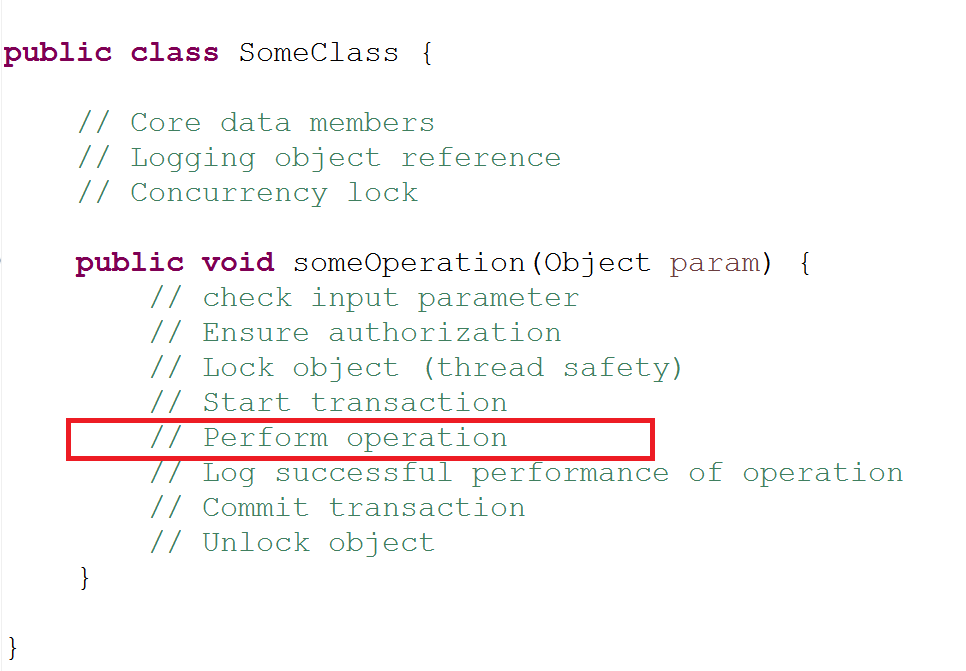
\includegraphics[scale=1.0]{bilder/motivationprogram.png}
	\caption{Beispielsklasse - Motivation für AOP}
	\label{fig:classmotivationaop}
\end{figure}



\paragraph{Code Tangling}

\paragraph{Code Scattering}

\subsection{Modularisierung mit AOP}
\label{sec:aop_modaop}


\section{Aspektorientierte Sprache}
\label{sec:aop_lang}

\subsection{Spezifizierung}

\subsection{Implementation}

\section{Konzepte}

\section{Programmiersprachen}

\paragraph{Java}

\paragraph{.NET Framework}

\paragraph{C++}
